\documentclass[addpoints,12pt]{exam}
\usepackage[]{graphicx}\usepackage[]{color}
%% maxwidth is the original width if it is less than linewidth
%% otherwise use linewidth (to make sure the graphics do not exceed the margin)
\makeatletter
\def\maxwidth{ %
  \ifdim\Gin@nat@width>\linewidth
    \linewidth
  \else
    \Gin@nat@width
  \fi
}
\makeatother

\definecolor{fgcolor}{rgb}{0.345, 0.345, 0.345}
\newcommand{\hlnum}[1]{\textcolor[rgb]{0.686,0.059,0.569}{#1}}%
\newcommand{\hlstr}[1]{\textcolor[rgb]{0.192,0.494,0.8}{#1}}%
\newcommand{\hlcom}[1]{\textcolor[rgb]{0.678,0.584,0.686}{\textit{#1}}}%
\newcommand{\hlopt}[1]{\textcolor[rgb]{0,0,0}{#1}}%
\newcommand{\hlstd}[1]{\textcolor[rgb]{0.345,0.345,0.345}{#1}}%
\newcommand{\hlkwa}[1]{\textcolor[rgb]{0.161,0.373,0.58}{\textbf{#1}}}%
\newcommand{\hlkwb}[1]{\textcolor[rgb]{0.69,0.353,0.396}{#1}}%
\newcommand{\hlkwc}[1]{\textcolor[rgb]{0.333,0.667,0.333}{#1}}%
\newcommand{\hlkwd}[1]{\textcolor[rgb]{0.737,0.353,0.396}{\textbf{#1}}}%


\usepackage{alltt}
\usepackage{mathtools}
%%\usepackage{marginnote}
%%\usepackage[top=1in, bottom=1in, outer=5.5in, inner=1in, heightrounded, marginparwidth=1in, marginparsep=1in]{geometry}
\usepackage{enumerate}
%% mess with the fonts
%%\usepackage{fontspec}
%%\defaultfontfeatures{Ligatures=TeX} % To support LaTeX quoting style
\usepackage[T1]{fontenc}
\usepackage[utf8]{inputenc}
% For package xtable
\usepackage{booktabs}  % Nice toprules and bottomrules
\heavyrulewidth=1.5pt  % Change the default to heavier lines
\usepackage{longtable} 
%%\usepackage{tabularx}  % To control the width of the table
% this should make caption font bold.
%%\usepackage{xstring}
%%\usepackage{etoolbox}
%%\usepackage{url}
%% xetex only \usepackage{breakurl}
\usepackage{float} % for fig.pos='H'
%%\usepackage{wrapfig}
%%\usepackage{tikz}
\usepackage{colortbl,xcolor}

\newcommand{\dev}[1] {Dev_{\bar{#1}}}

\IfFileExists{upquote.sty}{\usepackage{upquote}}{}
\begin{document}
\header{Math 2300 Section 2}{Exam 1}{February 27, 2015}
\begin{center}
\fbox{\fbox{\parbox{5.5in}{\centering
Please answer the questions in the spaces provided on the
question sheets. If you run out of room for an answer,
continue on the back of the page. Please show all work for maximum credit.}}}
\end{center}
\vspace{0.1in}
\makebox[\textwidth]{Name:\enspace\hrulefill}
%\pointsinmargin
\bracketedpoints

\begin{questions}

\question
A group of six friends has median age 21. Five of the ages are 18, 24, 20, 19, and 25.
\begin{parts}
\part[5]
What is the age of the sixth friend?
\vspace{1cm}
\part[5]
What is the mean age of the six friends?
\vspace{1cm}
\part[5]
Suppose the 25 year old friend leaves the group, and a new friend aged 23 joins the group, does the median age of the group of friends change? 
\part[5] Does the mean age change? 
\end{parts}
\question
Holderness Elementary School has a weather station that tracks Temperature in \textdegree F, Dewpoint in \textdegree F, Barometric Pressure in Inches, and Windspeed in MPH. Summary statistics and covariances are:
\vspace{5mm}
\begin{table}[ht]
\centering
\begin{tabular}{rrrrr}
  \hline
 & TemperatureF & DewpointF & PressureIn & WindSpeedMPH \\ 
  \hline
  Min. & -20.70 & -25.00 & 29.00 & 0.00 \\ 
  Max. & 17.30 & 1.00 & 29.40 & 3.00 \\ 
  Median & 8.20 & -7.00 & 29.30 & 0.00 \\ 
  Mean & 1.40 & -10.80 & 29.20 & 0.68 \\ 
  Variance & 177.40 & 71.00 & 177.40 & 71.00 \\ 
  Standard Deviation & 13.30 & 8.40 & 13.30 & 8.40 \\ 
   \hline
\end{tabular}
\end{table}
\begin{table}[ht]
\centering
\begin{tabular}{rrrrr}
  \hline
 & & Covariance & Association Measure\\ 
  \hline
Temperature & Dewpoint & 107.79 & \\
Temperature & Pressure & -1.32 & \\
Temperature & Windspeed & 4.69 & \\ 
Dewpoint & Pressure & -0.98 & \\
Dewpoint & Windspeed & 1.50 & \\ 
Pressure & Windspeed &  0.02 & \\ 
   \hline
\end{tabular}
\end{table}
\begin{parts}
\part[10] What is the most suitable measure to quantify the association between each of the variables? 
\vspace{1cm}
\part[10] Calculate your chosen measure of association and add it to the chart.
\vspace{1cm}
\part[10] Do any pairs seem to be strongly associated? Briefly discuss.
\vspace{2cm}
\end{parts}
\titledquestion{June Ice Cream Sales}
An ice cream stand opened for the season in June. For each of the first ten days, the daily high temperature in \textdegree F was recorded with the daily sales in dollars.
\begin{table}[ht]
\centering
\begin{tabular}{rrrrrrrrrrr}
  \hline
Day & 3 & 1 & 4 & 2 & 10 & 5 & 8 & 7 & 6 & 9 \\ 
  \hline
High Temp &  53 &  58 &  59 &  62 &  63 &  65 &  65 &  67 &  72 &  73 \\ 
  Sales & 185 & 215 & 332 & 325 & 408 & 406 & 421 & 412 & 522 & 445 \\ 
   \hline
\end{tabular}
\caption{Temperature and Sales for the first ten days in June, sorted by Temperature}
\end{table}
\vspace{1cm}
\begin{parts}
\part[5] What was the median high temperature for the first ten days in June?
\vspace{1cm}
\part[5] What was the range in sales for the first ten days in June?
\vspace{1cm}
\end{parts}
\vspace{1cm}
The totals for deviation calculations are:
% latex table generated in R 3.1.2 by xtable 1.7-4 package
% Thu Feb 26 20:15:36 2015
\begin{table}[ht]
\centering
\begin{tabular}{rrrrrrrr}
  \toprule
 & Temp \textdegree F & Sales & $\dev{x}$ & $\dev{y}$ & $(\dev{x})^2$ & $(\dev{y})^2$ & $\dev{x}\dev{y}$ \\ 
 % \midrule
%3 &  53 & 185 & -182.0 & -10.7 & 33124.0 & 114.5 & 1947.4 \\ 
%   \rowcolor[gray]{0.95}1 &  58 & 215 & -152.0 & -5.7 & 23104.0 & 32.5 & 866.4 \\ 
%  4 &  59 & 332 & -35.0 & -4.7 & 1225.0 & 22.1 & 164.5 \\ 
%   \rowcolor[gray]{0.95}2 &  62 & 325 & -42.0 & -1.7 & 1764.0& 2.9 & 71.4 \\ 
%  10 &  63 & 408 & 41.0 & -0.7 & 1681.0 & 0.5 & -28.7 \\ 
%   \rowcolor[gray]{0.95}5 &  65 & 406 & 39.0 & 1.3 & 1521.0 & 1.7 & 50.7 \\ 
%  8 &  65 & 421 & 54.0 & 1.30 & 2916.0 & 1.7 & 70.2 \\ 
%   \rowcolor[gray]{0.95}7 &  67 & 412 & 45.0 & 3.3 & 2025.0 & 10.9 & 148.5 \\ 
%  6 &  72 & 522 & 155.0 & 8.3 & 24025.0 & 68.9 & 1286.5 \\ 
%   \rowcolor[gray]{0.95}8 &  73 & 445 & 78.0 & 9.3 & 6084.0 & 86.5 & 725.4 \\ 
%   \bottomrule
Total & 3671.0& 637.0&  0.0&  0.0& 97469.0& 342.2& 5302.3  \\ 
\rowcolor[gray]{0.95}& &  &   & & & & \\
\rowcolor[gray]{0.95}& &  &   & & & & \\
\rowcolor[gray]{0.95}& &  &   & & & & \\
\end{tabular}
\caption{Sales and Temperature for first ten days in June, sorted by Temperature} 
\end{table}
\begin{parts}
\begin{figure}[h]
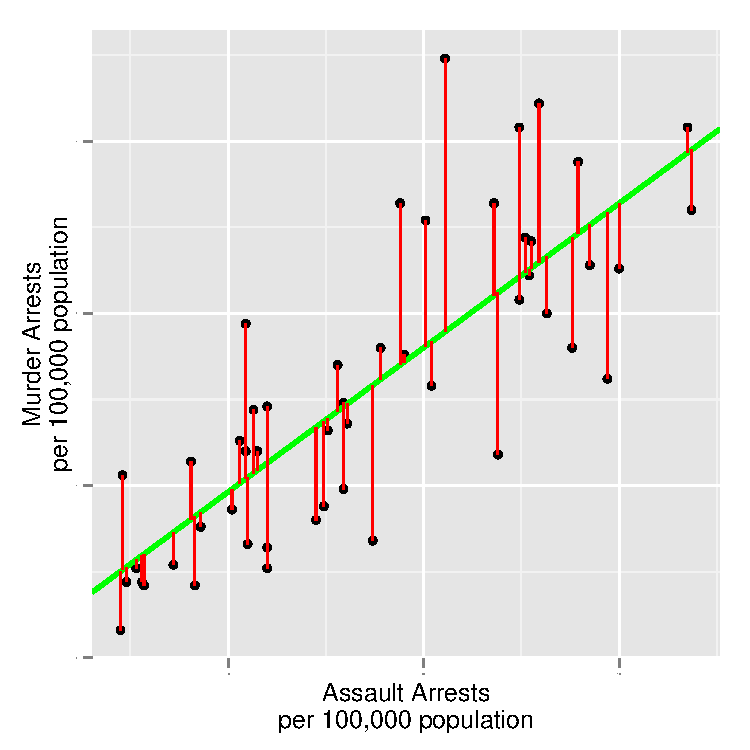
\includegraphics[width=\maxwidth]{figure/graphics-ols-1} 
\caption{Scatterplot of Temperature v Sales for June 1 through June 10}\label{fig:ols}
\end{figure}
\vspace{1cm}
\part[10] What is the correlation statistic between temperature and sales for these tens days? 
\vspace{1cm}
\part[10] Does there appear to be a linear correlation between the temperature and sales? If so, it the linear relationship positive or negative?
\vspace{3cm}
\part[10] Based on this data, what might be a reasonable change in sales dollars per degree F for these ten days?
\end{parts}
\newpage
\bonusquestion
\textbf{BONUS QUESTION}
\vspace{5mm}
The sales and high temperature for next eight days in June are:
\vspace{5mm}
\begin{table}[ht]
\centering
\begin{tabular}{rrrrrrrrr}
  \hline
 & 11 & 12 & 17 & 13 & 18 & 16 & 14 & 15 \\ 
  \hline
Temp &  74 &  77 &  82 &  88 &  91 &  93 &  94 &  95 \\ 
  Sales & 544 & 614 & 563 & 493 & 412 & 401 & 376 & 209 \\ 
   \hline
\end{tabular}
\caption{Temperature and Sales for June 11-18, sorted by Temperature}
\end{table}
% Thu Feb 26 21:57:36 2015
\vspace{5mm}
\begin{parts}
\bonuspart[5] What was the median high temperature for the first eighteen days in June?
\vspace{1cm}
\bonuspart[5] What was the range in sales for the first eighteen days in June?
\vspace{1cm}


\begin{table}[ht]
\centering
\begin{tabular}{rrrrrrrr}
  \toprule
 & Temp & Sales & $\dev{x}$ & $\dev{y}$ & $(\dev{x})^2$ & $(\dev{y})^2$ & $\dev{x}\dev{y}$ \\ 
%  \midrule
%9 &  74 & 544 & 92.00 & -12.80 & 8464.00 & 163.80 & -1177.60 \\ 
%   \rowcolor[gray]{0.95}8 &  77 & 614 & 162.00 & -9.80 & 26244.00 & 96.00 & -1587.60 %\\ 
%  17 &  82 & 563 & 111.00 & -4.80 & 12321.00 & 23.00 & -532.80 \\ 
%   \rowcolor[gray]{0.95}13 &  88 & 493 & 41.00 & 1.20 & 1681.00 & 1.40 & 49.20 \\ 
%  18 &  91 & 412 & -40.00 & 4.20 & 1600.00 & 17.60 & -168.00 \\ 
%   \rowcolor[gray]{0.95}16 &  93 & 401 & -51.00 & 6.20 & 2601.00 & 38.40 & -316.20 \\ 
%  14 &  94 & 376 & -76.00 & 7.20 & 5776.00 & 51.80 & -547.20 \\ 
%   \rowcolor[gray]{0.95}20 &  95 & 209 & -243.00 & 8.20 & 59049.00 & 67.20 & -1992.60 %\\ 
%   \bottomrule
Total & 3612.0& 694.0&  0.0&  0.0& 117736.0& 459.2& -6272.8  \\ 
\rowcolor[gray]{0.95}& &  &   & & & & \\
\rowcolor[gray]{0.95}& &  &   & & & & \\
\rowcolor[gray]{0.95}& &  &   & & & & \\
\rowcolor[gray]{0.95}& &  &   & & & & \\
\end{tabular}
\caption{Totals of Deviation table for June 11-June 18} 
\end{table}
\vspace{5mm}
\bonuspart[10]
What is the correlation between sales and temperature for all eighteen days?
\vspace{2cm}
\bonuspart[10]
Does this change any conclusions drawn from reviewing the first ten days only? Discuss.
\end{parts}

\end{questions}

\end{document}
